\chapter{Sistema \textit{True}}

Observando a realidade de um ambiente inteligente fica claro que as informações como posição das pessoas e suas respectivas identidades são imprescindíveis para que decisões possam ser tomadas. Atualmente, a maioria das soluções encontradas para fornecer esse tipo de informação foram projetadas para funcionar em ambientes rigidamente definidos. Com isso, não seria adequado tentar incorporar soluções como estas em um ambiente com diferentes dimensões, condições de iluminação, posição dos móveis, diferentes sensores pois este resultaria em um cenário diferente. Além disso, a solução deve ser integrada com o middleware \textit{UbiquitOS}, o qual gerência os serviços providos pelo ambiente inteligente.

Esse trabalho propõe, então, um sistema aberto de rastreamento, localização e identificação de pessoas em um ambiente inteligente integrado com o middleware \textit{UbiquitOS}. Tal sistema será chamado de TRUE, \textit{\textbf{T}racking and \textbf{R}ecognizing \textbf{U}sers in the \textbf{E}nvironment}.

O Sistema \textit{True} é um sistema monomodal que utiliza somente dados visuais, como imagens de cor e profundidade. As imagens de profundidade serão utilizadas no rastreamento e localização dos usuários no ambiente, e as imagens de cor serão utilizadas no reconhecimento facial e no cadastro dos usuários. Portanto, os dispositivos presentes no ambiente devem ser capazes de fornecer esses tipos de dados a um taxa e qualidade adequada. 

Para obter os dados necessários, o sistema utiliza o sensor \textit{Kinect} da Microsoft~\ref{sec:kinect}, um dispositivo bastante acessível e capaz de fornecer imagens de cor e de profundidade sincronizadas a uma taxa e qualidade necessária.

O sistema \textit{True} é dividido em três módulos principais:

	\begin{itemize}
		\item \textbf{Módulo de Rastreamento e Localização}: parte do sistema responsável pelo rastreamento e localização dos usuários no ambiente.
		\item \textbf{Módulo de Reconhecimento}: parte do sistema responsável por identificar os usuários rastreados.
		\item \textbf{Módulo de Registro}: parte do sistema responsável pelo cadastro de novos usuários e treino do sistema
	\end{itemize}

O Módulo de Registro será independente dos demais. Porém, os outros dois módulos devem trocar informações entre si para centralizar todas as informações (localização e reconhecimento) de todos usuários rastreados no ambiente. A seguir, é explicado mais detalhadamente cada módulo e como tal troca de informações ocorre.

No final deste capítulo, a integração do Sistema \textit{True} com o middleware \textit{UbiquitOS} é detalhada.

\section{Módulo de Reconhecimento}

	O Módulo de Reconhecimento, como se deduz do próprio nome, é responsável pela identificação dos usuários no ambiente utilizando a face como característica biométrica, pois ela permite um reconhecimento de forma não intrusiva, como mensionada na Seção~\ref{sec:biometria}. 

	Para realizar a detecção facial é utilizado o método \textit{Viola-Jones}~\ref{ref:viola-jones}. Um método que pode ser utilizado para construir uma abordagem de detecção facial rápida e eficaz~\cite{violajones} em tempo real. Além disso, este método é implementado pela biblioteca \textit{OpenCV} (\textit{Open Source Computer Vision}) onde bons classificadores em cascata de \textit{Haar features} são fornecidos, como por exemplo um classificador de faces frontais, utilizado nesse sistema.

	Para realizar o reconhecimento facial é utilizado \textit{Eigenfaces}~\ref{sec:reconhecimento}. Uma técnica bastante satisfatória quando utilizada sobre uma base de dados (faces) relativamente grande, permitindo ao sistema inferir, das imagens suas principais características e, partindo delas, realizar o reconhecimento das imagens utilizando um número bastante reduzido de cálculos~\cite{artigo-eigenface}, permitindo, assim, um reconhecimento em tempo real.

	A detecção e o reconhecimento são feitos em imagens de usuários que são passadas pelo Módulo de Rastreamento. Essa imagens são compostas somente pela região da imagem em que o usuário se encontra, como mostrado na Figura (\textbf{colocar figura aqui.}). Basicamente, o processo de reconhecimento é realizado pelas seguintes etapas e ilustrado na Figura~\ref{fig:processo-reconhecimento}:

		\begin{enumerate}
			\item Obtém a imagem de entrada correspondente a imagem formada somente pelo usuário cujo reconhecimento foi requisitado.
			\item Pré-processamento da imagem: a imagem é convertida em escala de cinza.
			\item Realiza detecção facial na imagem. Caso nenhuma face seja encontrada, retorna ``vazio''. Vale ressaltar que no máximo uma face pode ser encontrada nesta imagem.
			\item Processamento da imagem: uma nova imagem é criada recortando a região da face encontrada, a imagem, então, é redimensionada e equalizada criando assim uma padrão de tamanho, brilho e contraste nas imagens aumentando a acurácia do reconhecimento.
			\item Reconhecimento facial com \textit{Eigenfaces} é realizado.
			\item Retorna o nome da face ``mais parecida'' e a confiança do reconhecimento.
		\end{enumerate}

		\begin{figure}[hbt]
			\begin{center}
				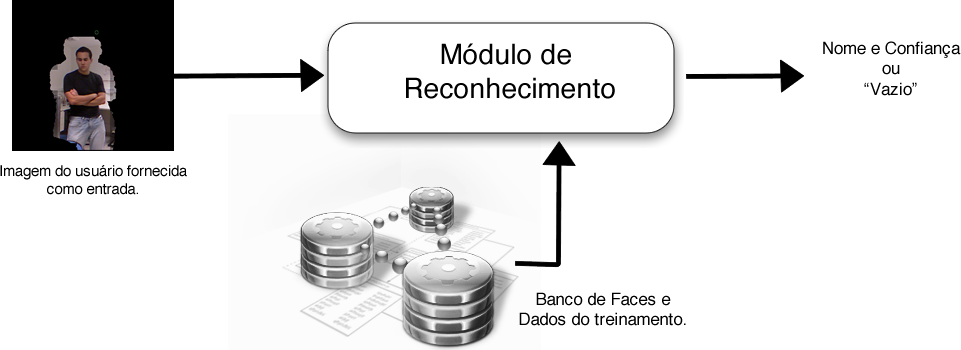
\includegraphics[scale=2.0]{figuras/4.ProblemaEProposta/reconhecimento-simples.png}
			\end{center}
			\caption{Representação das etapas propostas para o reconhecimento facial no Módulo de Reconhecimento.}
			\label{fig:processo-reconhecimento}
		\end{figure}

	O Módulo de Reconhecimento é dependente do de Rastreamento. Ele ficará ocioso até que chegue uma requisição de reconhecimento de um determinado usuário. A Seção~\ref{sec:rastreamento-reconhecimento} explica mais detalhadamente a relação entre os dois módulos.

	\subsection{Pré-processamento e Processamento da Imagem}
		
		As etapas de processamento das imagens permitem criar um padrão nas mesmas aumentando a acurácia do reconhecimento. No Sistema \textit{True} as etapas de processamento consistem em converter a imagem em escala de cinza, redimensiona-la e equaliaza-la criando, assim, um padrão de cor, tamanho, brilho e contraste nas imagens.

		A Figura~\ref{fig:greyscale} exemplifica uma imagem normal de uma face, depois a mesma convertida em escala de cinza e equalizada.

		\begin{figure}[hbt]
			\begin{center}
				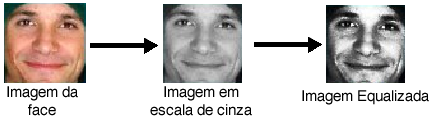
\includegraphics[scale=0.7]{figuras/4.ProblemaEProposta/greyscale.png}
			\end{center}
			\caption{Exemplo de uma imagem de face normal, em escala de cinza e equalizada. Adaptada de~\cite{shervin}.}
			\label{fig:greyscale}
		\end{figure}

	\subsection{Detecção Facial}

		O processo de detecção facial procura por uma face na imagem de entrada que já terá sido pré-processada, então estará em escala de cinza. Como já mencionado, a detecção facial é feita utilizando o método \textit{Viola-Jones} implementado pela biblioteca \textit{OpenCV}.

	\subsection{Reconhecimento Facial com \textit{Eigenfaces}}

\section{Módulo de Rastreamento}

	O Módulo de Rastreamento será responsável por rastrear os usuários no \textit{SmartSpace}, determinar a localização física de cada um em relação ao \textit{Kinect} e gerenciar suas identidades.

	Para realizar rastreamento e localização dos usuários será utilizado a implementação existente na biblioteca \textit{OpenNI} (\textit{Open Natural Interaction}). Trata-se de um \textit{framework} que define \textit{APIs} para o desenvolvimento de aplicações utilizando interação natural. Utilizando as imagens de profundidade, a detecção e o rastreamento dos usuários será feita utilizando subtração de fundo~\ref{sec:deteccao-objeto} e a representação dos usuários será feita por silhuetas~\ref{sec:representacao-objeto}. 

	O rastreamento e a localização serão feitas utilizando as imagens de profundidades providas pelo \textit{Kinect} obtidas utilizando o método de Luz Estruturada descrito na seção~\ref{sec:luz-estruturada}, tornando-os não susceptíveis as variações nas condições de iluminação. Essas imagens de profundidade nada mais são que \textit{depth maps} (mapas de profundidade), em que cada pixel da imagem contém o valor estimado da distância em relação ao sensor. O \textit{Kinect} fornece esses dados a uma taxa de $\displaystyle 30 fps$ (\textit{frames} por segundo) com uma resolução $\displaystyle 320px$ x $\displaystyle 240px$.
	
	Com esses mapas de profundidade, a biblioteca \textit{OpenNI} consegue calcular as coodernadas $\displaystle (x,y,z)$ em relação ao \textit{Kinect} de qualquer pixel na imagem. Ou seja, se tivermos a representação de um usuário rastreado na imagem, conseguiremos obter sua localização relativa ao \textit{Kinect} de cada pixel pertencente ao usuário. Então, fixando a posição do \textit{Kinect} no ambiente, conseguiremos estimar a localização de qualquer usuário rastreado em tempo real.

\section{Relação Rastreamento e Reconhecimento}
\label{sec:rastreamento-reconhecimento}

	Até agora, foi mostrado como os Módulos de Rastreamento e de Reconhecimento funcionarão de maneira isolada, mas não como irão se relacionar. O Módulo de Rastreamento irá deter as informações sobre todos os usuários rastreados no ambiente e será responsável por requisitar reconhecimento ao Módulo de Reconhecimento, que deverá acontecer quando um novo usuário for detectado ou quando for necessário reconhecer um usuário já rastreado.

	Basicamente, quando um novo usuário for detectado, a relação entre rastreamento e reconhecimento acontecerá de acordo com as seguintes etapas e representada na Figura~\ref{fig:rastreamento-reconhecimento}:

		\begin{figure}[hbt]
			\begin{center}
				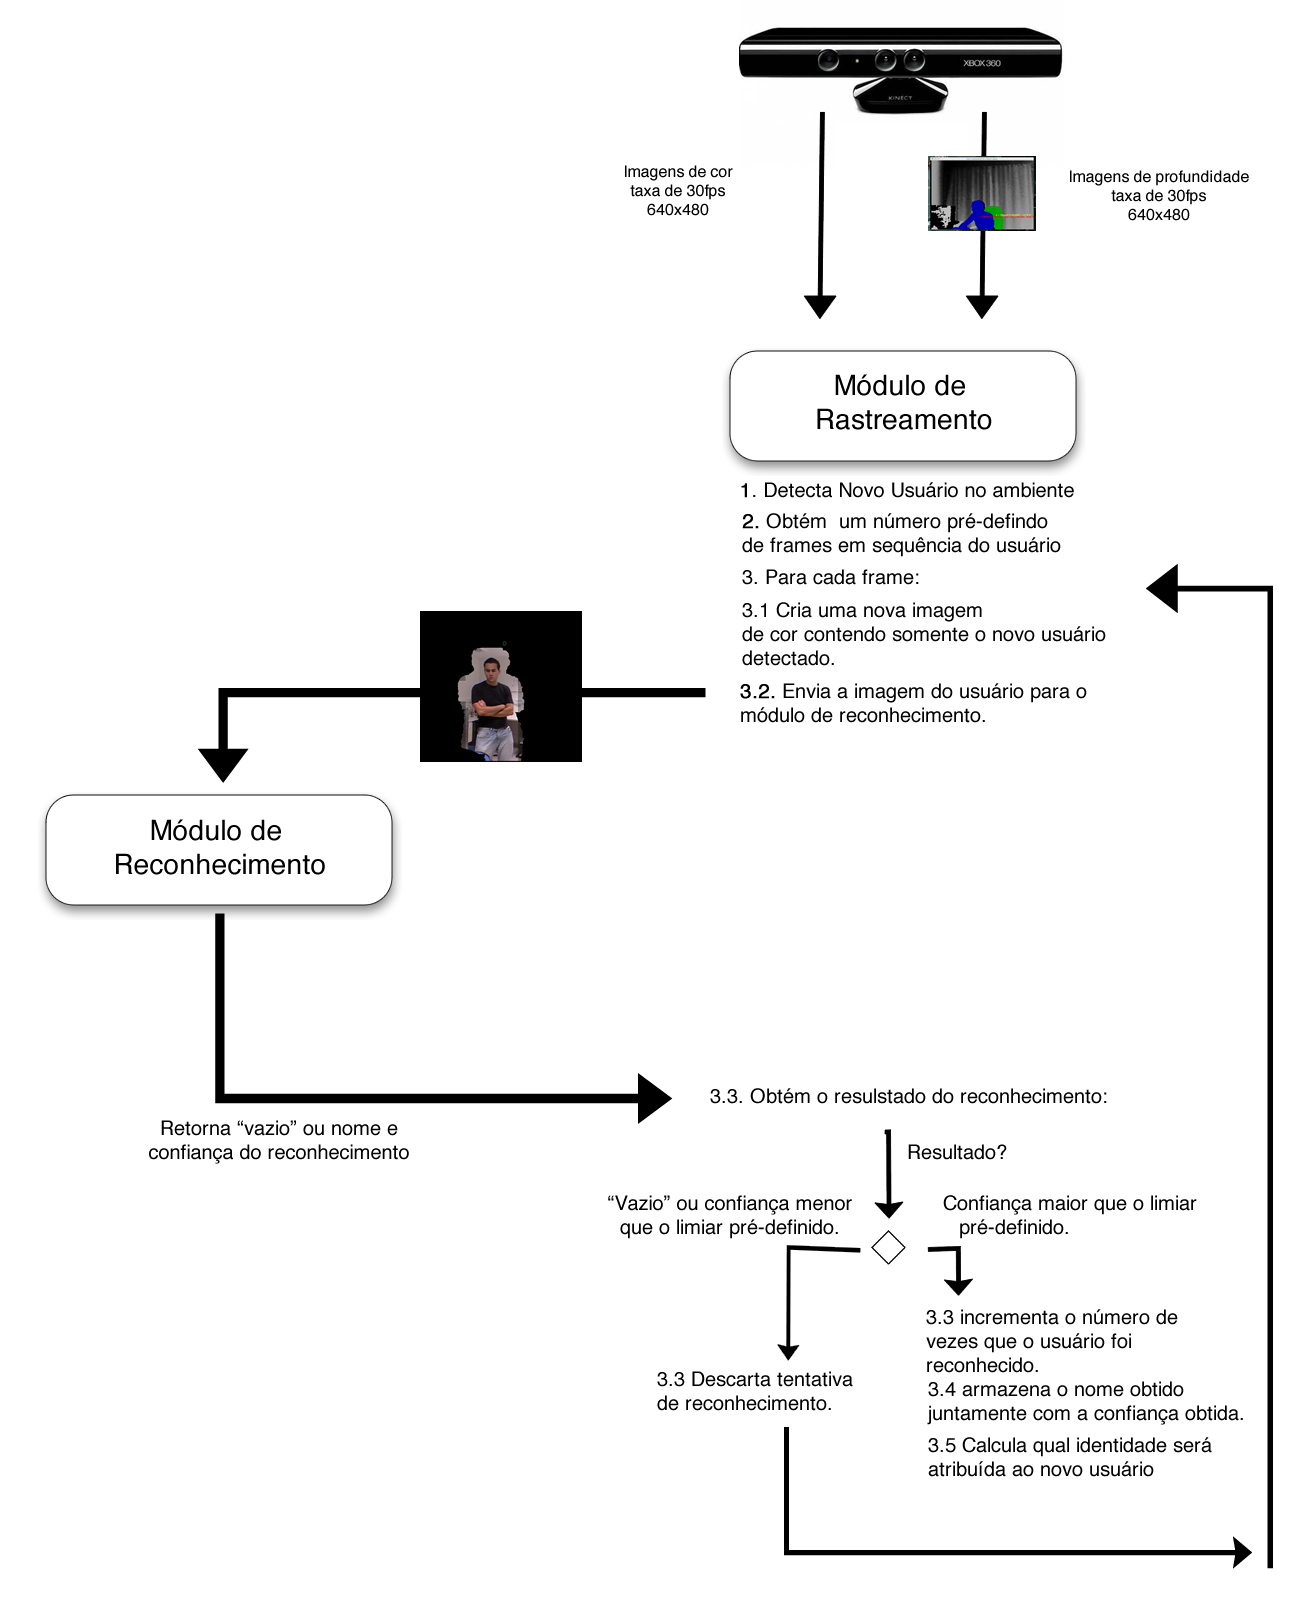
\includegraphics[scale=1.5]{figuras/4.ProblemaEProposta/esquema-tracker-reco.png}
			\end{center}
			\caption{Representação da relação que o Módulo de Rastreamento terá com o Módulo de Reconhecimento quando um novo usuário for detectado.}
			\label{fig:rastreamento-reconhecimento}
		\end{figure}
	
		\begin{enumerate}
		 	\item O Módulo de Rastreamento detecta novo usuário, e obtém um número pré-definido de imagens sucessivas do novo usuário. Para cada imagem, ele cria uma nova imagem de cor contendo somente aquele usuário, como mostrado na Figura (\textbf{colocar a figura aqui}), e a envia para o Módulo de Reconhecimento.
		 	\item Para cada imagem recebida, o Módulo de Reconhecimento tenta reconhecer o novo usuário e retorna ``vazio'' ou o nome e a confiança do reconhecimento.
		 	\item O Módulo de Rastreamento verifica se a confiança é maior que um limiar pré-definido, se for ele incrementa o contador que armazena o número de vezes que o usuário foi reconhecido, armazena o nome obtido juntamente com a confiança e calcula qual nome  será atribuído ao novo usuário. Esse cálculo será feito por meio de uma média ponderada utilizando os diferentes resultados obtidos por cada reconhecimento e suas respectivas confianças.
	 	\end{enumerate} 
	
	Ao invés de tentar realizar o reconhecimento somente quando novos usuários são detectados, o sistema \textit{True} continuará a tentar reconhecer os usuários já reconhecidos para melhorar a confiança no reconhecimento. Essas tentativas de reconhecer novamente os usuários ocorrerão em intervalos de tempo pré-definidos seguindo as mesmas etapas de quando um novo usuário for detectado. A única etapa que será diferente será a primeira: ao invés de obter várias imagens de um mesmo usuário, serão obtidas uma imagem de cada usuário rastreado e as mesmas serão enviadas ao Módulo de Reconhecimento.

	Desta maneira, o Módulo de Rastreamento conseguirá reunir em um só lugar todas as informações sobre os usuários rastreados, como localização corrente, nome, confiança do reconhecimento, quantas vezes o usuário foi reconhecido e quais diferentes nomes foi atribuído ao mesmo.

\section{Módulo de Registro}

	O Módulo de Registro será responsável por cadastrar novos usuários no sistema e treiná-lo para também reconhecer esse novo usuário. Basicamente, o processo de registro seguirá as seguintes etapas e ilustrada na Figura~\ref{fig:registro}:

		\begin{figure}[hbt]
			\begin{center}
				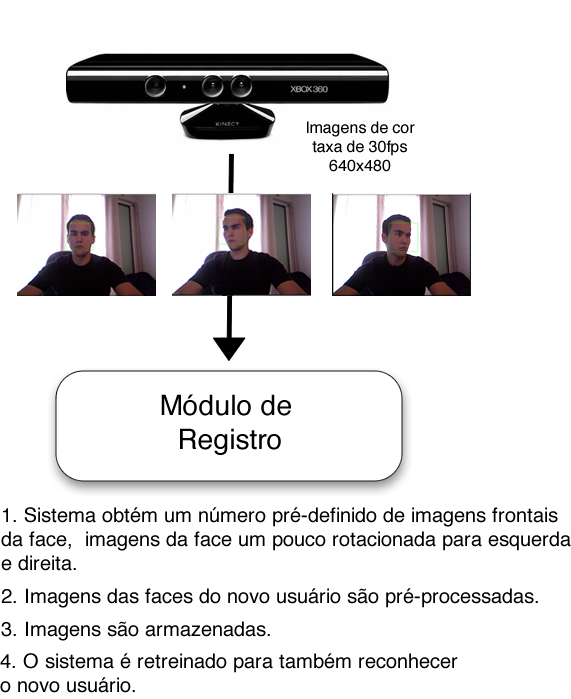
\includegraphics[scale=2.5]{figuras/4.ProblemaEProposta/registro.png}
			\end{center}
			\caption{Etapas de cadastro de um novo usuário no sistema.}
			\label{fig:registro}
		\end{figure}		

		\begin{enumerate}
			\item O novo usuário fica em uma posição fixa e frontal em relação ao \textit{Kinect}. 
			\item O sistema obtém um número pré-definido de imagens frontais do usuário.
			\item O usuário, então, deve rotacionar um pouco a face para a esquerda e o sistema obtém um número pré-definido de imagens do usuário. Depois, deve rotacionar um pouco para direita e o sistema obtém mais imagens do usuário.
			\item As imagens obtidas são processadas: as imagens são convertidas em escala de cinza, novas imagens são criadas recortando a região da face encontrada, as imagens, então, são redimensionadas e equalizadas criando assim uma padrão de tamanho, brilho e contraste nas imagens.
			\item Armazena-se as imagens.
			\item O sistema é treinado para, também, reconhecer esse usuário.
		\end{enumerate}

	Após o treinamento, o sistema \textit{True} reiniciará para que o reconhecimento seja feito utilizando as novas informações obtidas com o treinamento.

\section{\textit{SmartSpace} Laico}

	O ambiente para o qual o sistema \textit{True} será projetado, desenvolvido e testado chama-se LAICO (\textbf{LA}boratório de sistemas \textbf{I}ntegrados e \textbf{CO}ncorrente), um laboratório do Departamento de Ciência da Computação da Universidade de Brasília. O LAICO possui dimensões de, aproximadamente,  $\displaystyle 7,67m$ x $\displaystyle 6,45m$ ilustrado pela Figura~\ref{fig:laico}.

	\begin{figure}[hbt]
			\begin{center}
				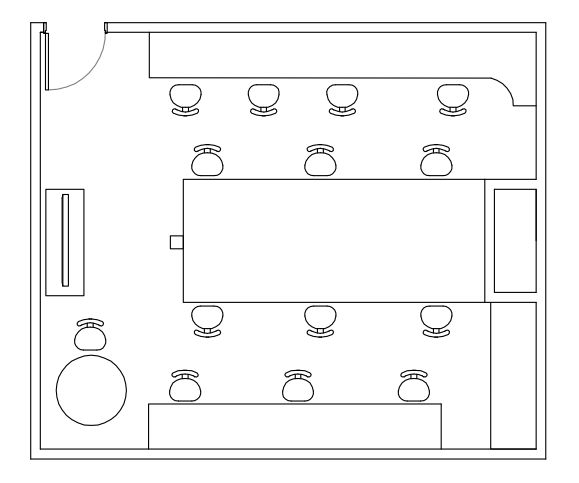
\includegraphics[scale=0.6]{figuras/4.ProblemaEProposta/laico.png}
			\end{center}
			\caption{Planta do \textit{SmartSpace} Laico.}
			\label{fig:laico}
		\end{figure}	














